\documentclass[11pt]{article}

\usepackage{fancyhdr}
\usepackage{hyperref}
\usepackage{graphicx}

\graphicspath{ {images/} }
 
\pagestyle{fancy}
\fancyhf{}
\lhead{University of the Witwatersrand}
\rfoot{School of Computer Science and Applied Mathematics}
\pagenumbering{roman}

\begin{document}

\begin{titlepage}

\newcommand{\HRule}{\rule{\linewidth}{0.3mm}} % Defines a new command for the horizontal lines, change thickness here
\renewcommand\section{\@startsection{section}{1}{\z@}%
                                  {-3.5ex \@plus -1ex \@minus -.2ex}%
                                  {2.3ex \@plus.2ex}%
                                  {\normalfont\large\bfseries}}

\center % Center everything on the page
 
%----------------------------------------------------------------------------------------
%	HEADING SECTIONS
%----------------------------------------------------------------------------------------

\textsc{\LARGE University of the Witwatersrand}\\[1.5cm] % Name of your university/college
\textsc{\Large School of Computer Science and Applied Mathematics}\\[0.5cm] % Major heading such as course name

%----------------------------------------------------------------------------------------
%	TITLE SECTION
%----------------------------------------------------------------------------------------

\HRule \\[0.4cm]
{ \huge \bfseries COMS3007: Machine Learning Assingment}\\[0.4cm] % Title of your document \\
  \large 13 May 2016
\HRule \\[1.5cm]
 
%----------------------------------------------------------------------------------------
%	AUTHOR SECTION
%----------------------------------------------------------------------------------------
\begin{minipage}{1\textwidth}
	\Large \emph By Chalom, J. (711985)\\
\end{minipage}


\vfill % Fill the rest of the page with whitespace

\end{titlepage}
\begin{page}
\section{Purpose}
The purpose of my assignment is to run several machine learning algorithms in order to correctly classify hand written digits as their corresponding ASCII equivalents, or at least predict within an acceptable order of magnitude. These sets of experiments will hopefully show that machine learning can be applied to the field of optical character recognition.

\section{Tools Used}
I made used of the node.js framework for my coding and scripting of the various experiments. I used the Synaptic neural network library for node.js. This library was capable of handling constructing the given dimensions of a network, changing relevant values, randomising the data and calculating the error during training. \url{http://synaptic.juancazala.com/}

\section{Dataset Used}
I made use of the MNIST database. This is a large database of hand written digits which has been compiled by taking a combination of two databases of hand written digits compiled in the United States. The website for this database can be found here: \url{http://yann.lecun.com/exdb/mnist/} \\

This database has a very large training set of 60 000 examples and a set of 10 000 test examples. All the images are normalised, and centred in the same fixed size of 28x28 pixels.
I used the mnist library for node.js to help me load the database into Synaptic. It can be found here: https://github.com/cazala/mnist \\\\

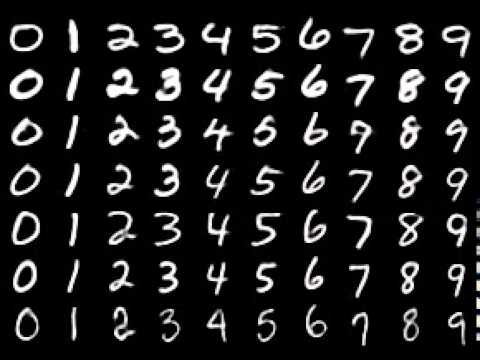
\includegraphics[scale=0.7]{1}\\
An example of the data used (several sets of samples compiled together) \\
Source: \url{https://github.com/cazala/mnist/}\\

Using this library I was able to specify the number of training samples and testing samples I wanted. No two sets are the same using the functionality of this library. I specified 700 training examples and 20 testing examples. \\\\

My neural networks all had 784 input nodes (which correspond per pixel to the input image samples) and 10 output nodes (which correspond to the digits 0-9) as my attributes of classification. My networks setup using Synaptic JS accept a 784 length array of values (floats) and outputs a 10 length array of values (floats). I run the test data on the network after training and round the output values to the nearest integer after the network. \\\\

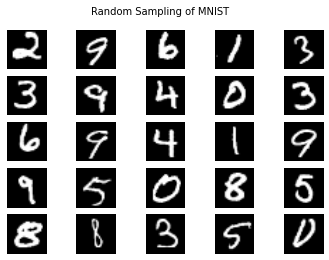
\includegraphics{2}\\
This is an example of a randomly sampled data:\\
Source: \url{http://ampcamp.berkeley.edu/6/exercises/} 

\section{General Restrictions and Normalisation Applied}


\section{Algorithms Used}
\emph Note: See results for the error returned on the test set.\\\\
 
Synaptic runs multiple iterations of each network when training. Each iteration randmosies the data so the error has variation, each iteration. On all experiments I ran 10 iterations (detailed in Results).\\\\

\textbf{Experiment 1:} Neural network with one hidden layer with 100 nodes and learning rate of 0.3\\\\
\textbf{Experiment 2:} Neural network with two hidden layers with 50 nodes on each layer and a learning rate of 0.3\\\\
\textbf{Experiment 3:} Neural network with three hidden layers with 25 nodes on each layer and a learning rate of 0.3\\\\
\textbf{Experiment 4:} Neural network with three hidden layers with 50 nodes on each layer and a learning rate of 0.3\\\\
\textbf{Experiment 5:} Neural network with two hidden layers with 50 nodes on each layer and a learning rate of 0.2\\\\
\textbf{Experiment 6:} Neural network with three hidden layers with 20 nodes on each layer and a learning rate of 0.2\\\\
\textbf{Experiment 7:} Neural network with three hidden layers with 25 nodes on layer 1, 50 modes on layer, 25 nodes on layer 3 and a learning rate of 0.3\\\\
\textbf{Experiment 8:} RBF network with 25 RBF nodes and random centres and a learning rate of 0.3\\\\

\section{Results}

\textbf{Experiment 1:} \\\\

\\
\textbf{Experiment 2:} \\\\

\\
\textbf{Experiment 3:} \\\\

\\
\textbf{Experiment 4:} \\\\

\\
\textbf{Experiment 5:} \\\\

\\
\textbf{Experiment 6:} \\\\

\\
\textbf{Experiment 7:} \\\\

\\
\textbf{Experiment 8:} \\\\

\\

\section{Conclusion}
A brief discussion of your results from the various algorithms. E.g., what worked best/worst
and why you think this is so.\\

\section{Discussion}

\end{page}
\end{document}
